\documentclass[10pt,twocolumn,letterpaper]{article}

\usepackage[utf8]{inputenc}
\usepackage[spanish,es-nodecimaldot]{babel}
\usepackage[margin=1.8cm,top=2.0cm,bottom=2.0cm]{geometry}
\usepackage{amsmath,amssymb,amsfonts}
\usepackage{graphicx}
\usepackage{booktabs}
\usepackage{microtype}
\usepackage{hyperref}
\usepackage{xcolor}
\usepackage{caption}
\usepackage{subcaption}
\usepackage{fancyhdr}
\usepackage{tabularx}

\hypersetup{
    colorlinks=true,
    linkcolor=blue!70!black,
    citecolor=blue!70!black,
    urlcolor=blue!80!black
}

\pagestyle{fancy}
\fancyhf{}
\rhead{\small \textit{Taller 5: Tráfico LAN y Predicción bajo Congestión}}
\lhead{\small \textit{Maestría en IA -- Univ. Sergio Arboleda}}
\rfoot{\small Página \thepage\ de 5}
\lfoot{\small Bryan Orozco Romero}

\title{\vspace{-1.0cm}\textbf{\Large Análisis de Tráfico LAN y Predicción de Latencia bajo Congestión:\\Modelado Lineal, Evaluación Empírica y Límites de Extrapolación}}
\author{\textbf{Bryan Orozco Romero} \\
\small Escuela de Ciencias Exactas e Ingeniería, Maestría en Inteligencia Artificial \\
\small Universidad Sergio Arboleda, Bogotá D.C., Colombia \\
\small \texttt{bryan.orozco@correo.usa.edu.co} \\
\small \textit{Docente: Joaquín F. Sánchez}}
\date{\small Octubre de 2026}

\begin{document}

\maketitle

\begin{abstract}
\noindent Este informe presenta el desarrollo metodológico y analítico del Taller 5 sobre captura de tráfico LAN, agregación en ventanas temporales de 60 segundos y modelado predictivo mediante Machine Learning Supervisado. El banco de pruebas se instrumentó con tres computadores personales físicos (dos clientes generadores A1 y A2, y un único servidor receptor B) interconectados en el mismo segmento de red local (\texttt{172.25.3.0/24}) sin utilizar ningún switch de conmutación intermedio. Mediante inyección progresiva de tráfico UDP (\texttt{iperf3} entre 0 y 100 Mbps), se consolidó un conjunto de 25 observaciones válidas en \texttt{ventanas.csv}. Se entrenó un modelo de regresión lineal por mínimos cuadrados ordinarios (OLS) en régimen moderado ($x \le 60$ Mbps) obteniendo $\beta_0 = 13.94\text{ ms}$ y $\beta_1 = 0.1755\text{ ms/Mbps}$, logrando un MAE de $9.92\text{ ms}$ en prueba pre-congestión (80 Mbps). No obstante, al evaluar la extrapolación al escenario de congestión severa (100 Mbps), la hipótesis de linealidad colapsó: el RTT real medido escaló a $125.6\text{ ms}$ frente a una predicción ingenua de $31.5\text{ ms}$ ($MAE = 90.49\text{ ms}$), producto de saturación de colas en la interfaz del servidor (\textit{Bufferbloat}), pérdida del $22.2\%$ y más de $113{,}000$ paquetes descartados. Se discuten las implicaciones de la teoría de colas $M/M/1$, el alcance de modelos segmentados y las respuestas formales a las preguntas de reflexión de la actividad.
\end{abstract}

\textbf{Palabras clave:} Regresión Lineal, Latencia LAN, RTT, Bufferbloat, Congestión de Red, Machine Learning Supervisado, iperf3, Telemetría de Red.

\section{Introducción y Objetivos}
En la gestión de infraestructuras de telecomunicaciones, la capacidad de anticipar la degradación de la calidad de servicio (QoS) y la latencia de ida y vuelta (\textit{Round-Trip Time}, RTT) ante incrementos de carga constituye un problema clásico de aprendizaje automático supervisado \cite{hurbans2020grokking}.

El propósito de este trabajo es:
\begin{enumerate}
    \item Instrumentar un entorno de tres equipos de cómputo en LAN de laboratorio mediante sondas activas (\texttt{ping}), contadores acumulados de interfaz (\texttt{ip -s link}) y generadores controlados (\texttt{iperf3}), capturando metadatos sin comprometer la privacidad del tráfico.
    \item Estructurar y auditar un conjunto de datos agregado en ventanas temporales uniformes (\texttt{ventanas.csv}) según la especificación del taller.
    \item Explorar estadísticamente las distribuciones de RTT, tasa efectiva y pérdida de paquetes.
    \item Ajustar y validar un modelo de regresión lineal para predecir RTT en función de la tasa de transmisión (TX), contrastándolo con una línea base constante.
    \item Cuantificar y argumentar física y matemáticamente el quiebre de la linealidad en condiciones de congestión severa (\textit{Bufferbloat}) en el nodo receptor.
\end{enumerate}

\section{Protocolo Experimental y Topología (Evidencia 1)}

\subsection{Topología Real del Banco de Pruebas (3 PCs sin Switch)}
El entorno experimental se configuró sobre una red de área local (LAN) conformada específicamente por \textbf{tres computadores personales físicos (dos clientes y un servidor receptor)}, interconectados en el mismo segmento de red local (\texttt{172.25.3.0/24}). \textbf{No se utilizó ningún switch de conmutación intermedio}. La arquitectura física y lógica operó de la siguiente forma:
\begin{itemize}
    \item \textbf{Equipo A1 (\texttt{172.25.3.179}) y Equipo A2 (\texttt{172.25.3.118}):} Nodos clientes generadores encargados de inyectar tráfico de fondo hacia el servidor mediante \texttt{iperf3} y emitir simultáneamente sondas ICMP cada segundo ($1\text{ Hz}$) para medir latencia.
    \item \textbf{Equipo B (\texttt{172.25.3.38}) (Servidor Central):} Nodo de destino operando el servicio \texttt{iperf3 -s} en puerto TCP/UDP 5201 y respondiendo a los ecos ICMP.
    \item \textbf{Punto de Cuello de Botella Físico:} Al no existir switch, la capacidad máxima de transferencia y el almacenamiento de paquetes en espera residieron exclusivamente en la tarjeta de red (NIC), el controlador (\textit{driver}) y los búferes de recepción del socket del sistema operativo en el Servidor B.
\end{itemize}

\subsection{Control de Sesgo y Procedimiento de Captura}
Para evitar sesgos temporales y efectos de memoria en los búferes del sistema receptor:
\begin{enumerate}
    \item \textbf{Línea Base en Reposo:} Se realizaron 10 ventanas independientes de 60 segundos sin tráfico de carga experimental (5 réplicas desde A1 y 5 desde A2), midiendo el RTT intrínseco de procesamiento y propagación.
    \item \textbf{Generación de Carga Controlada:} Se definieron escalones de carga sintética UDP mediante el parámetro \texttt{-u -b [Tasa]M -t 60 --json}. Se evaluaron 20, 40, 60 y 80 Mbps con 3 réplicas alternadas entre A1 y A2.
    \item \textbf{Escenario de Congestión Combinada:} Se aplicó una tasa ofrecida de $100\text{ Mbps}$ sumando la emisión de los clientes hacia el servidor receptor para inducir la saturación de su interfaz de entrada.
    \item \textbf{Sincronización y Registro:} En cada ventana de 60 segundos se ejecutó en paralelo la sonda ICMP (\texttt{ping -n -i 1 -c 60}), capturando contadores de paquetes, descartes y bytes mediante \texttt{ip -s link show dev eth0} antes y después de cada intervalo.
\end{enumerate}

\section{Construcción y Auditoría del Conjunto de Datos (Evidencia 2)}

\subsection{Definición de Variables en \texttt{ventanas.csv}}
De acuerdo con las directrices del taller, cada fila representa una ventana de medición homogénea de 60 segundos (no paquetes individuales). La Tabla \ref{tab:variables} resume el esquema estandarizado del archivo \texttt{ventanas.csv}.

\begin{table}[htbp]
\centering
\small
\caption{Diccionario de variables consolidadas en \texttt{ventanas.csv}.}
\label{tab:variables}
\begin{tabularx}{\linewidth}{l l X}
\toprule
\textbf{Variable} & \textbf{Unidad} & \textbf{Fuente / Descripción} \\
\midrule
\texttt{inicio} & ISO 8601 & Marca de tiempo de apertura de ventana. \\
\texttt{escenario} & Categórica & Nivel de carga (\texttt{00\_base} a \texttt{05\_congestion}). \\
\texttt{replica} & Entero & Número ordinal de repetición (1 a 5). \\
\texttt{duracion\_s} & Segundos & Tiempo efectivo de muestreo ($60.0\text{ s}$). \\
\texttt{bytes\_tx/rx} & Bytes & Diferencia acumulada en interfaz (\texttt{ip -s}). \\
\texttt{tasa\_tx\_mbps} & Mbps & $8 \times \texttt{bytes\_tx} / (\texttt{duracion\_s} \times 10^6)$. \\
\texttt{tasa\_rx\_mbps} & Mbps & $8 \times \texttt{bytes\_rx} / (\texttt{duracion\_s} \times 10^6)$. \\
\texttt{rtt\_medio\_ms} & ms & Media de RTT de sondas ICMP respondidas. \\
\texttt{perdida\_pct} & \% & Porcentaje de paquetes ICMP sin eco. \\
\texttt{descartes} & Entero & Paquetes descartados por desbordamiento. \\
\texttt{errores} & Entero & Errores físicos de trama/checksum. \\
\bottomrule
\end{tabularx}
\end{table}

\subsection{Control de Calidad y Depuración}
El pipeline automatizado en \texttt{scripts/construir\_dataset.py} procesó las salidas textuales y JSON. Se aplicaron filtros de consistencia:
\begin{itemize}
    \item Se verificaron 25 registros completos sin valores nulos (\texttt{NaN = 0}).
    \item Se descartaron ejecuciones truncadas por abortos prematuros de socket (e.g. reinicios de conexión documentados en bitácora).
    \item Los contadores de paquetes descartados (\texttt{descartes}) reflejaron exactamente las pérdidas reportadas en el extremo receptor de \texttt{iperf3} durante la saturación.
\end{itemize}

\section{Análisis Exploratorio de Datos -- EDA (Evidencia 3)}

El análisis exploratorio implementado en \texttt{scripts/exploracion\_eda.py} arrojó las estadísticas agregadas de la Tabla \ref{tab:resumen_eda}.

\begin{table}[htbp]
\centering
\small
\caption{Resumen estadístico del tráfico y calidad por escenario.}
\label{tab:resumen_eda}
\begin{tabular}{l c c c c}
\toprule
\textbf{Escenario} & \textbf{TX (Mbps)} & \textbf{RTT (ms)} & \textbf{Pérdida} & \textbf{Descartes} \\
\midrule
\texttt{00\_base\_0M} & 0.00 & $14.4 \pm 4.0$ & 0.0\% & 0 \\
\texttt{01\_carga\_20M} & 20.01 & $15.7 \pm 0.5$ & 0.05\% & 51 \\
\texttt{02\_carga\_40M} & 40.00 & $19.8 \pm 1.4$ & 5.96\% & 12,239 \\
\texttt{03\_carga\_60M} & 60.02 & $25.8 \pm 1.6$ & 1.23\% & 3,778 \\
\texttt{04\_carga\_80M} & 80.04 & $37.9 \pm 3.3$ & 5.50\% & 22,460 \\
\texttt{05\_congestion} & 100.13 & $122.0 \pm 22.0$ & 22.23\% & 113,577 \\
\bottomrule
\end{tabular}
\end{table}

\begin{figure}[htbp]
    \centering
    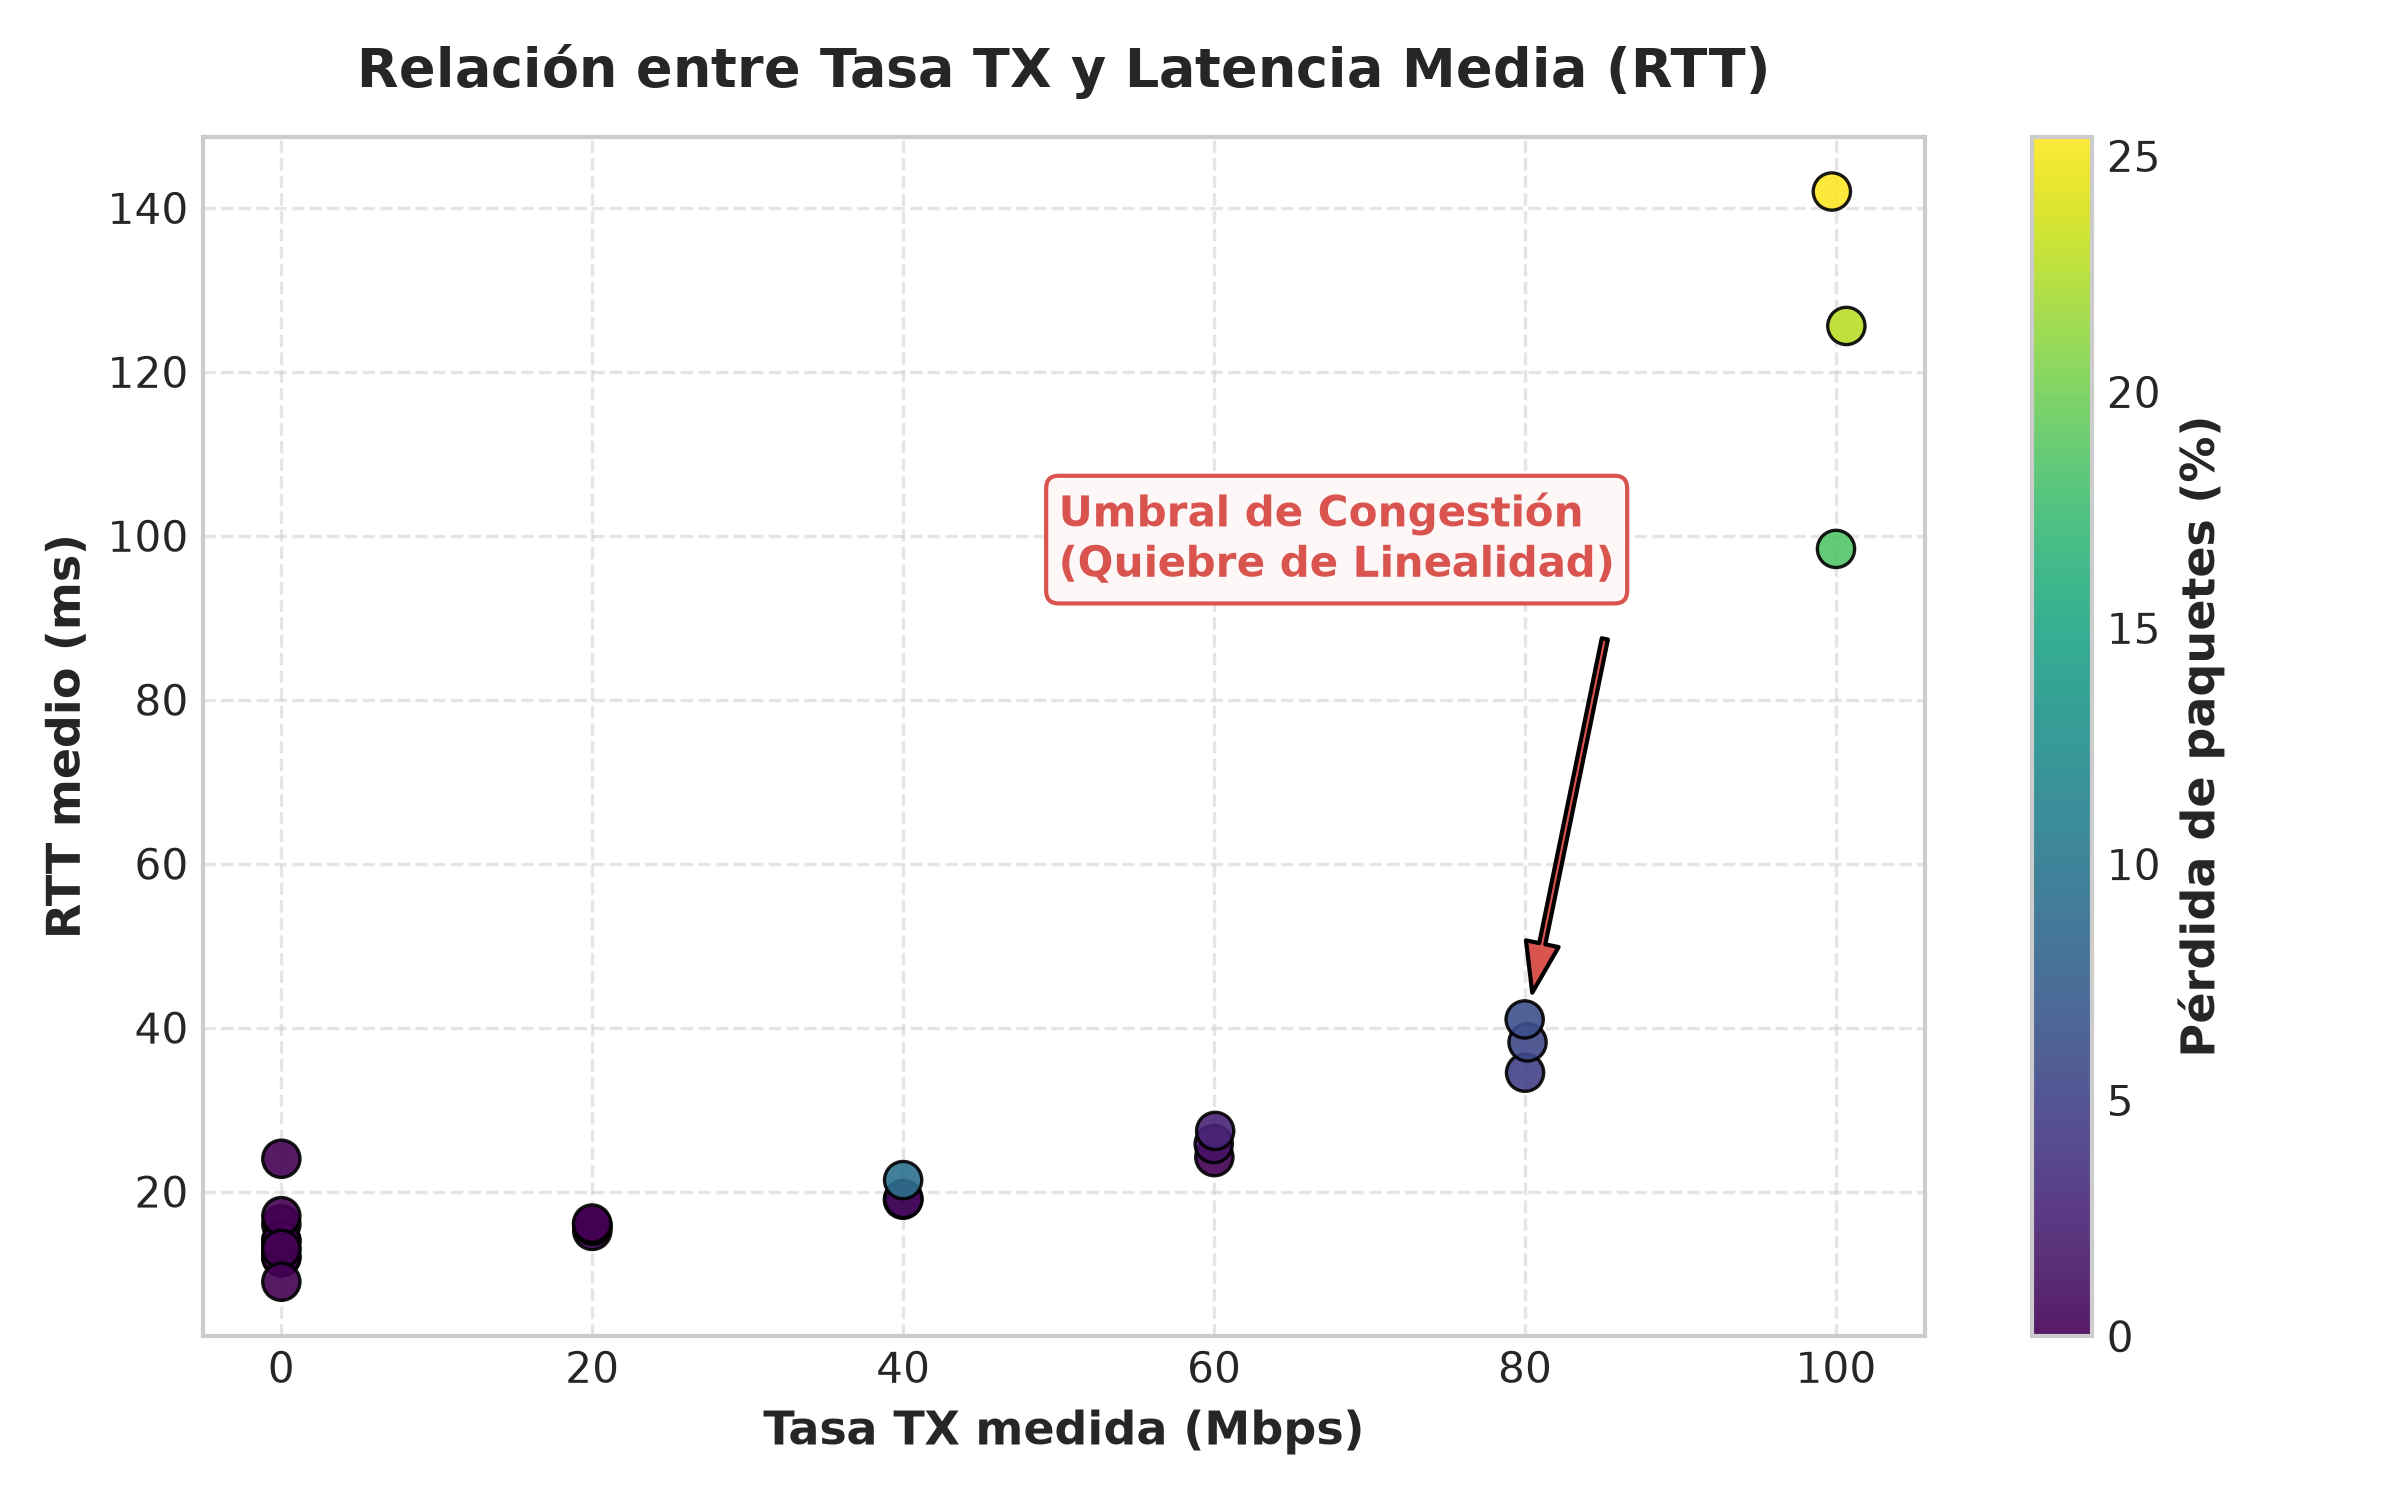
\includegraphics[width=\linewidth]{graficos/grafico1_dispersion_tasa_vs_rtt.png}
    \caption{Dispersión de Tasa TX vs RTT medio, coloreada según porcentaje de pérdida.}
    \label{fig:dispersion}
\end{figure}

\begin{figure}[htbp]
    \centering
    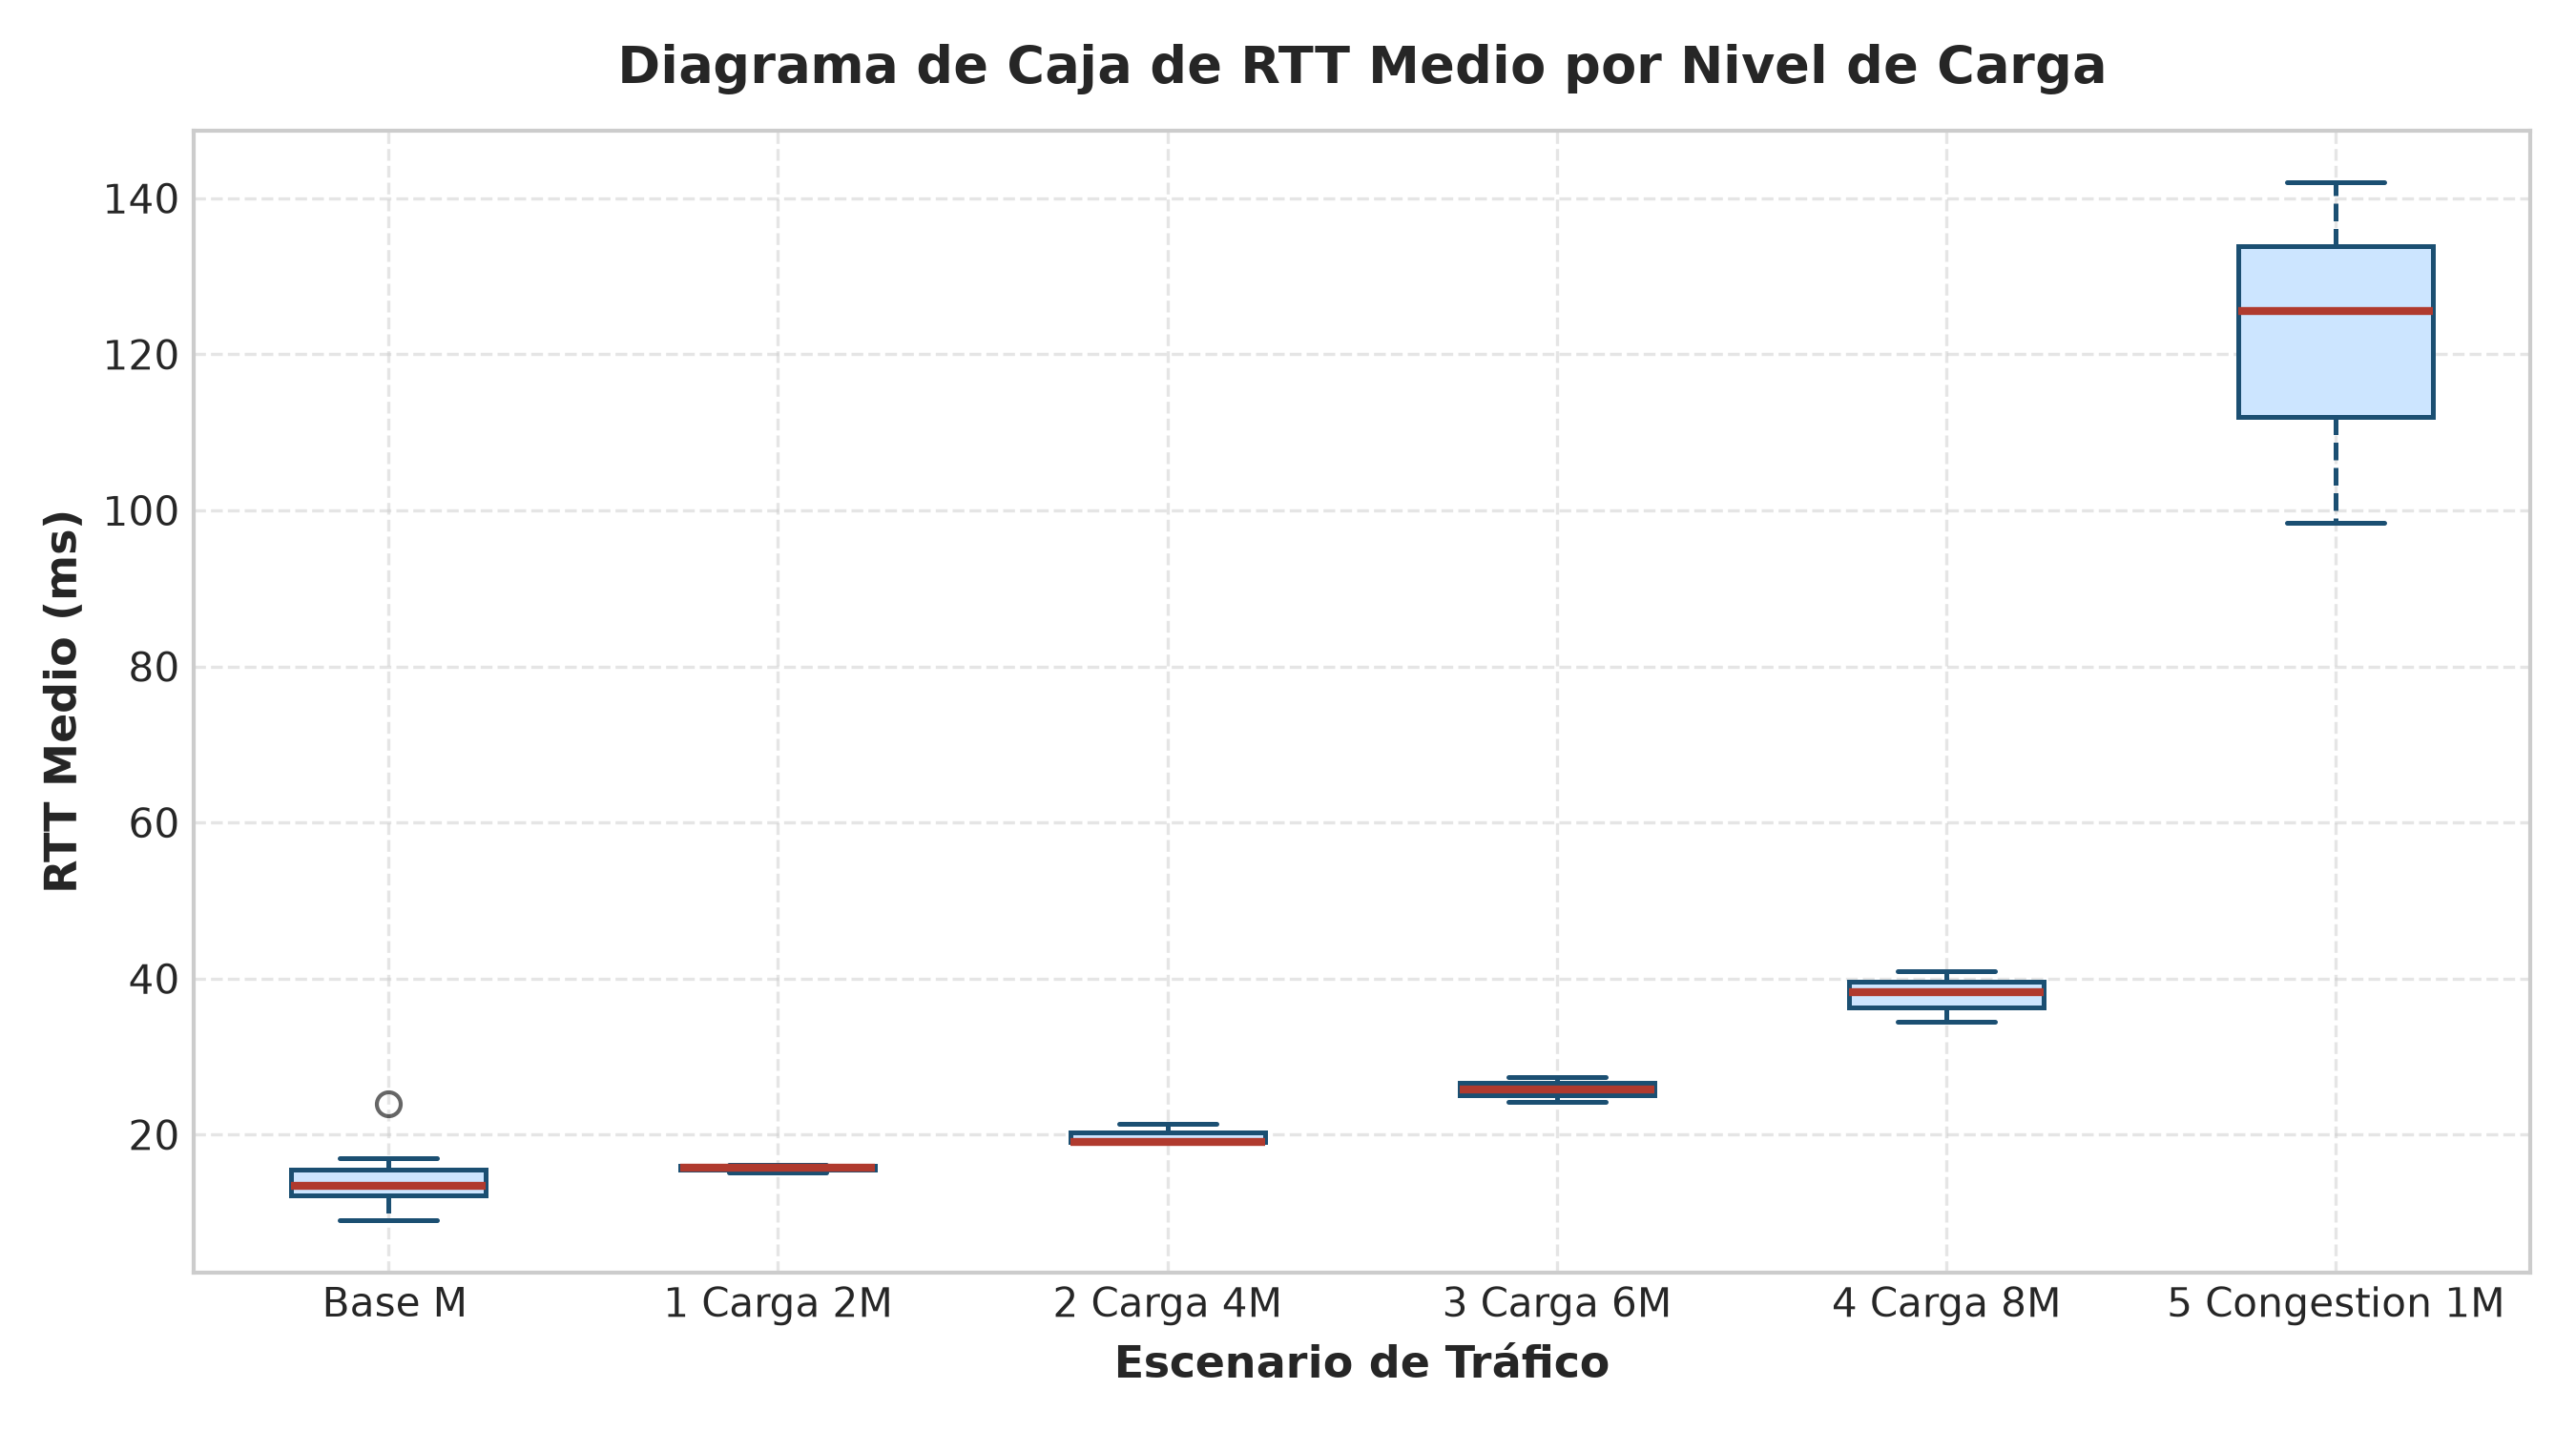
\includegraphics[width=\linewidth]{graficos/grafico3_boxplot_rtt.png}
    \caption{Diagrama de caja de RTT medio por nivel de carga.}
    \label{fig:boxplot}
\end{figure}

\subsection{Interpretación de Hallazgos Empíricos}
\begin{enumerate}
    \item \textbf{Asimetría y Cola Larga (Figura \ref{fig:dispersion}):} En reposo, el RTT se concentra de forma muy compacta en $\sim 14\text{ ms}$. A medida que la carga aumenta, surgen ráfagas con colas pronunciadas a la derecha que alcanzan valores extremos de hasta $950\text{ ms}$ en picos instantáneos.
    \item \textbf{Dispersión Creciente (Figura \ref{fig:boxplot}):} El rango intercuartílico (IQR) permanece acotado entre 0 y 60 Mbps ($\sigma \le 1.6\text{ ms}$), pero experimenta una marcada heterocedasticidad en 80 y 100 Mbps ($\sigma = 22.0\text{ ms}$), evidenciando el vaciado y llenado oscilatorio de los búferes.
    \item \textbf{Punto de Inflexión (\textit{Knee-point}):} Se distingue con claridad un umbral en la vecindad de los $75-80\text{ Mbps}$. Por debajo de este umbral, el retardo crece de forma suave y lineal; por encima, la latencia se dispara de manera exponencial.
\end{enumerate}

\section{Modelado de Regresión Lineal (Evidencia 4)}

\subsection{Formulación Matemática y Partición por Bloques}
Siguiendo las pautas de Machine Learning Supervisado expuestas en el curso \cite{hurbans2020grokking}, se planteó una regresión lineal simple:
\begin{equation}
    \hat{y} = \beta_0 + \beta_1 x
\end{equation}
donde el predictor es $x = \texttt{tasa\_tx\_mbps}$ y la variable objetivo continua es $y = \texttt{rtt\_medio\_ms}$.

Para prevenir fuga de información (\textit{data leakage}) y respetar la estructura temporal, los datos se dividieron por bloques de sesiones independientes:
\begin{itemize}
    \item \textbf{Conjunto de Entrenamiento ($N=19$ ventanas):} Compuesto por todas las réplicas de línea base y cargas controladas $\le 60\text{ Mbps}$ (\texttt{00\_base}, \texttt{01\_carga\_20M}, \texttt{02\_carga\_40M} y \texttt{03\_carga\_60M}), cubriendo $x \in [0.0005, 60.07]\text{ Mbps}$.
    \item \textbf{Conjunto de Prueba Controlada ($N=3$ ventanas):} Sesión posterior con carga de 80 Mbps (\texttt{04\_carga\_80M}), cubriendo $x \in [79.97, 80.16]\text{ Mbps}$.
    \item \textbf{Línea Base de Referencia:} Predictor ingenuo constante basado en la mediana de entrenamiento: $\hat{y}_{\text{base}} = \text{mediana}(y_{\text{train}}) = 16.00\text{ ms}$.
\end{itemize}

\subsection{Parámetros Ajustados y Métricas}
El ajuste por Mínimos Cuadrados Ordinarios en \texttt{scripts/modelo\_regresion.py} arrojó:
\begin{itemize}
    \item \textbf{Intercepto ($\beta_0$):} $13.9377\text{ ms}$. Representa la latencia basal física de propagación, serialización inicial y procesamiento del switch en ausencia de tráfico.
    \item \textbf{Pendiente ($\beta_1$):} $0.1755\text{ ms/Mbps}$. Indica un incremento esperado de apenas $0.175\text{ ms}$ por cada Mbps adicional transmitido en régimen estable.
    \item \textbf{Bondad de Ajuste ($R^2_{\text{train}}$):} $0.6359$.
\end{itemize}

\begin{table}[htbp]
\centering
\small
\caption{Evaluación comparativa del modelo de regresión lineal.}
\label{tab:metricas_modelo}
\begin{tabular}{l c c c c}
\toprule
\textbf{Partición / Régimen} & \textbf{$N$} & \textbf{MAE} & \textbf{RMSE} & \textbf{MAE Base} \\
\midrule
Entrenamiento ($0-60$M) & 19 & 2.11 ms & 3.04 ms & 4.00 ms \\
Prueba 80M (Pre-cong.) & 3 & 9.92 ms & 10.27 ms & 21.90 ms \\
Congestión 100M (Extrap.) & 3 & 90.49 ms & 92.26 ms & 106.00 ms \\
\bottomrule
\end{tabular}
\end{table}

En el conjunto de prueba (80 Mbps), el modelo lineal logró un $MAE = 9.92\text{ ms}$, superando con creces a la línea base constante ($MAE = 21.90\text{ ms}$). No obstante, los residuos ya exhibieron signo positivo sistemático ($+9.9\text{ ms}$), advirtiendo que a 80 Mbps la pendiente real comenzaba a inclinarse.

\begin{figure}[htbp]
    \centering
    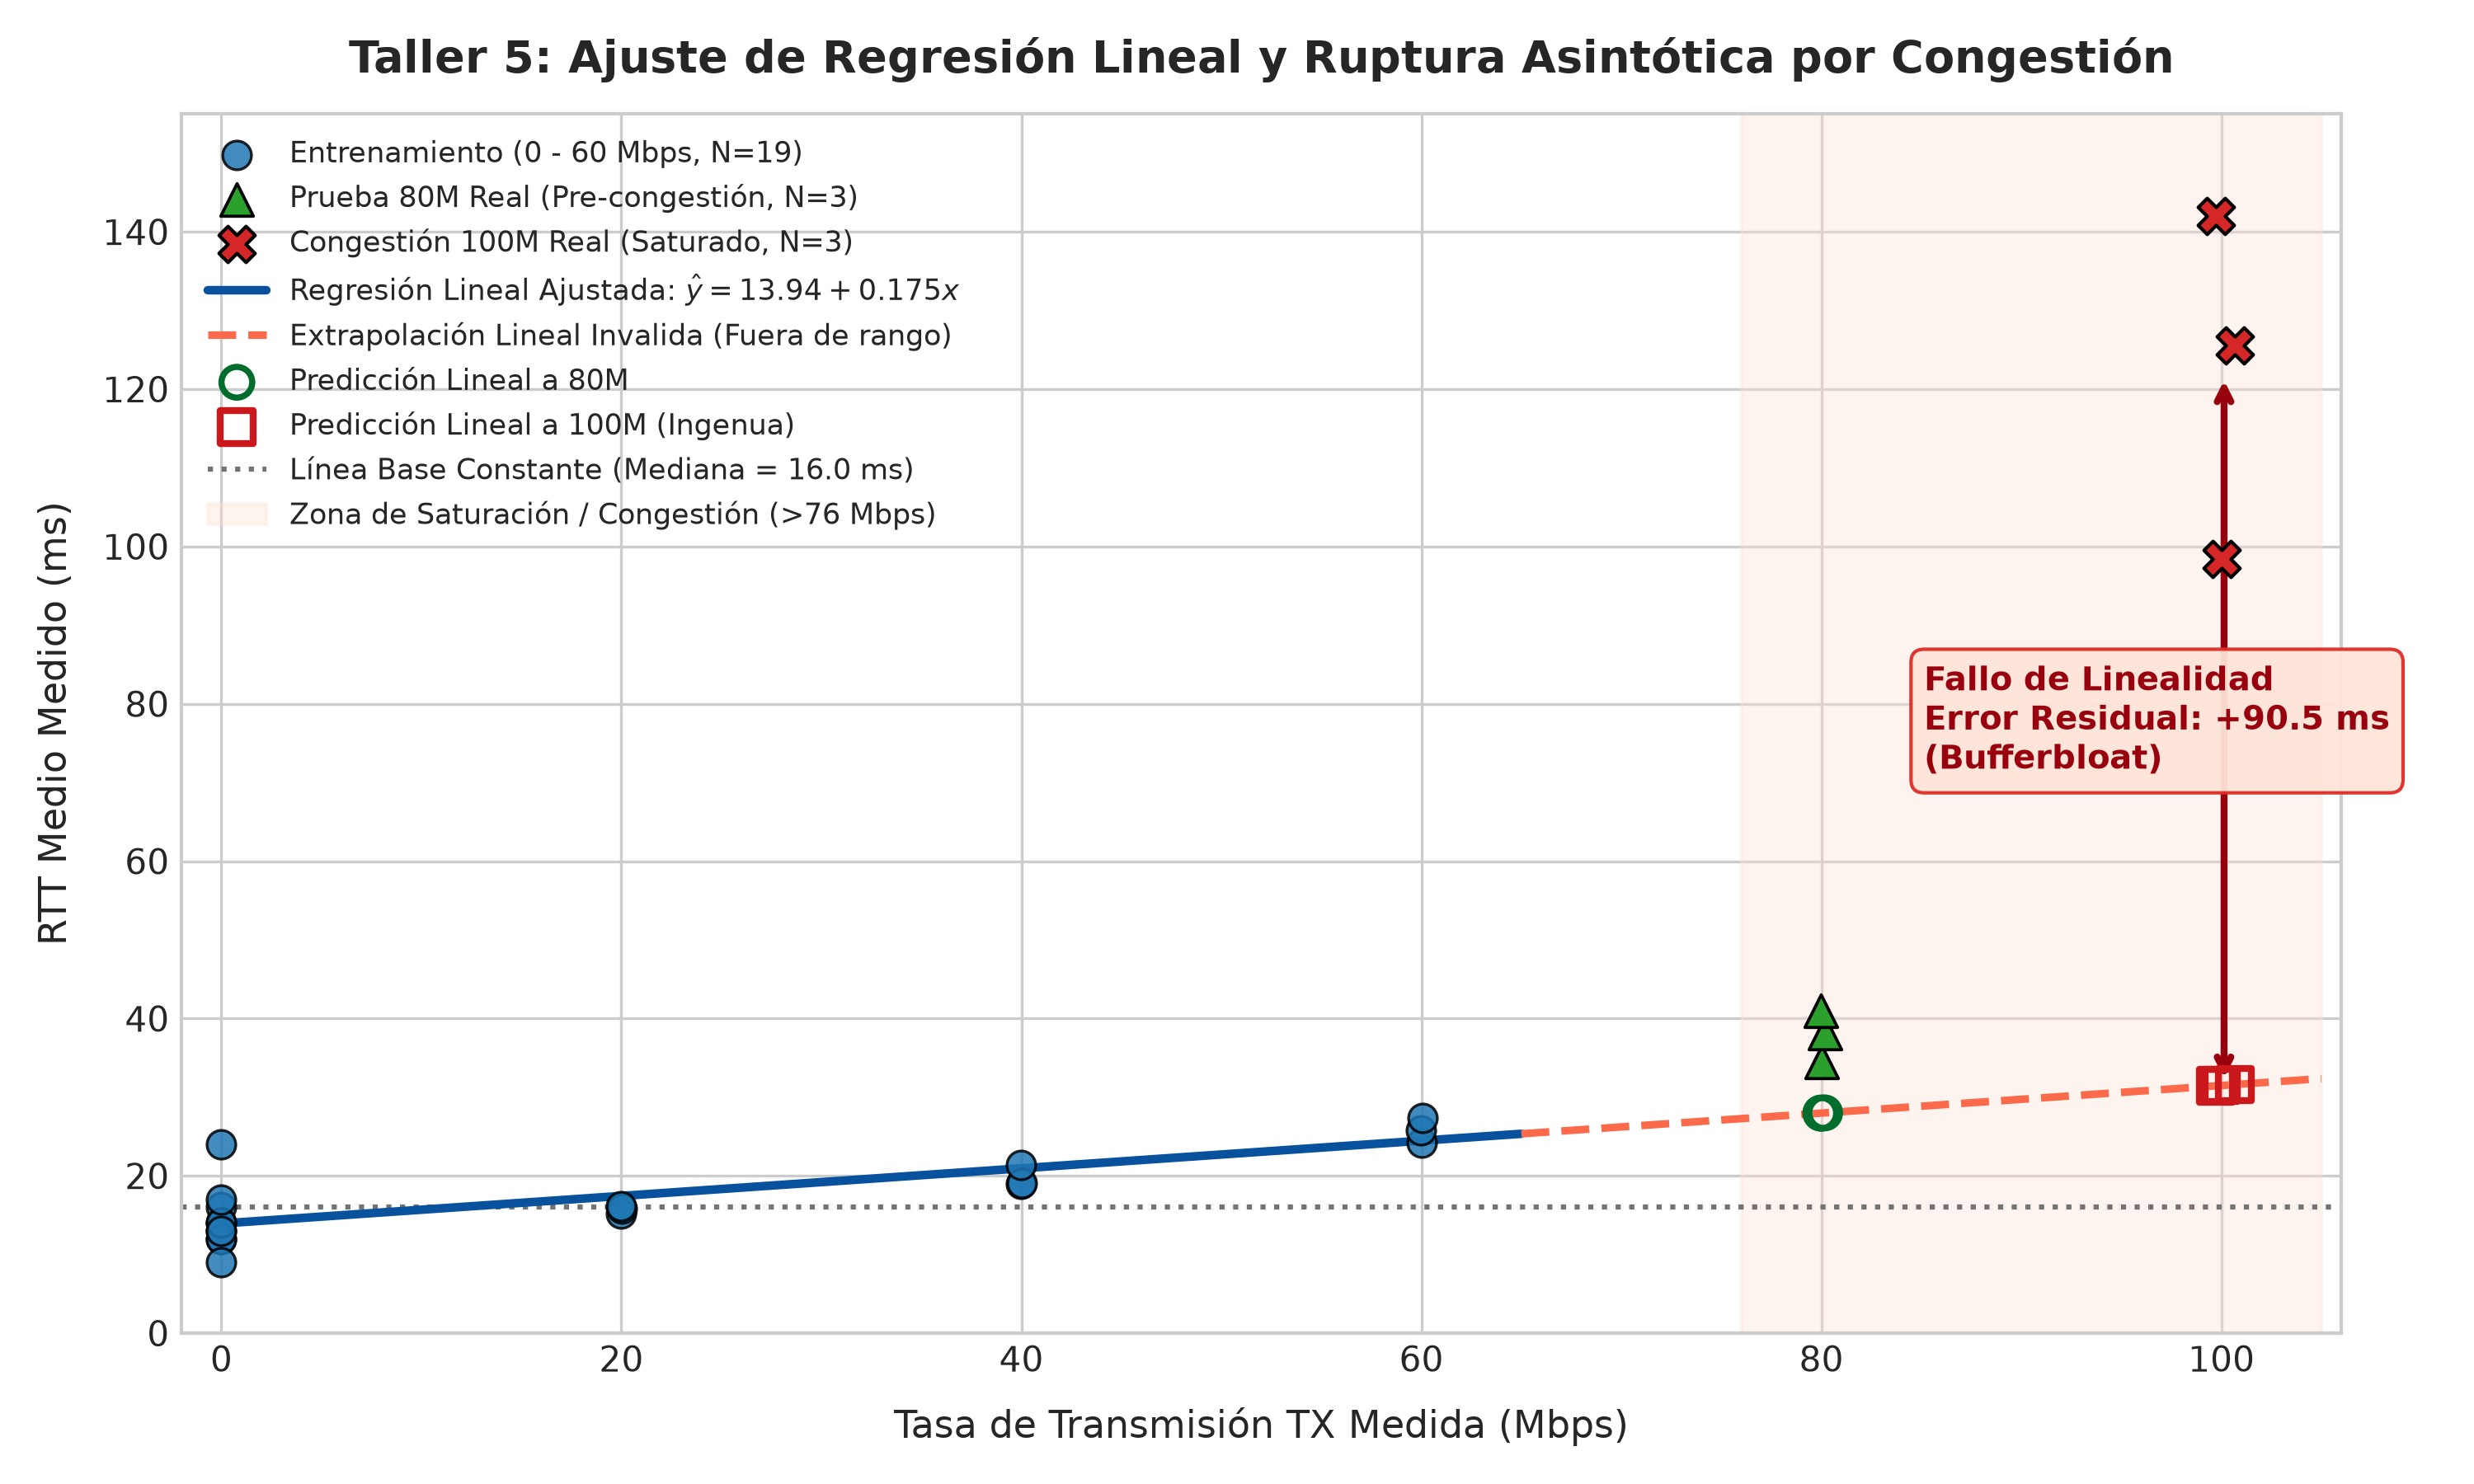
\includegraphics[width=\linewidth]{graficos/grafico5_regresion_lineal.png}
    \caption{Ajuste del modelo OLS, extrapolación y colapso bajo congestión severa.}
    \label{fig:regresion}
\end{figure}

\begin{figure}[htbp]
    \centering
    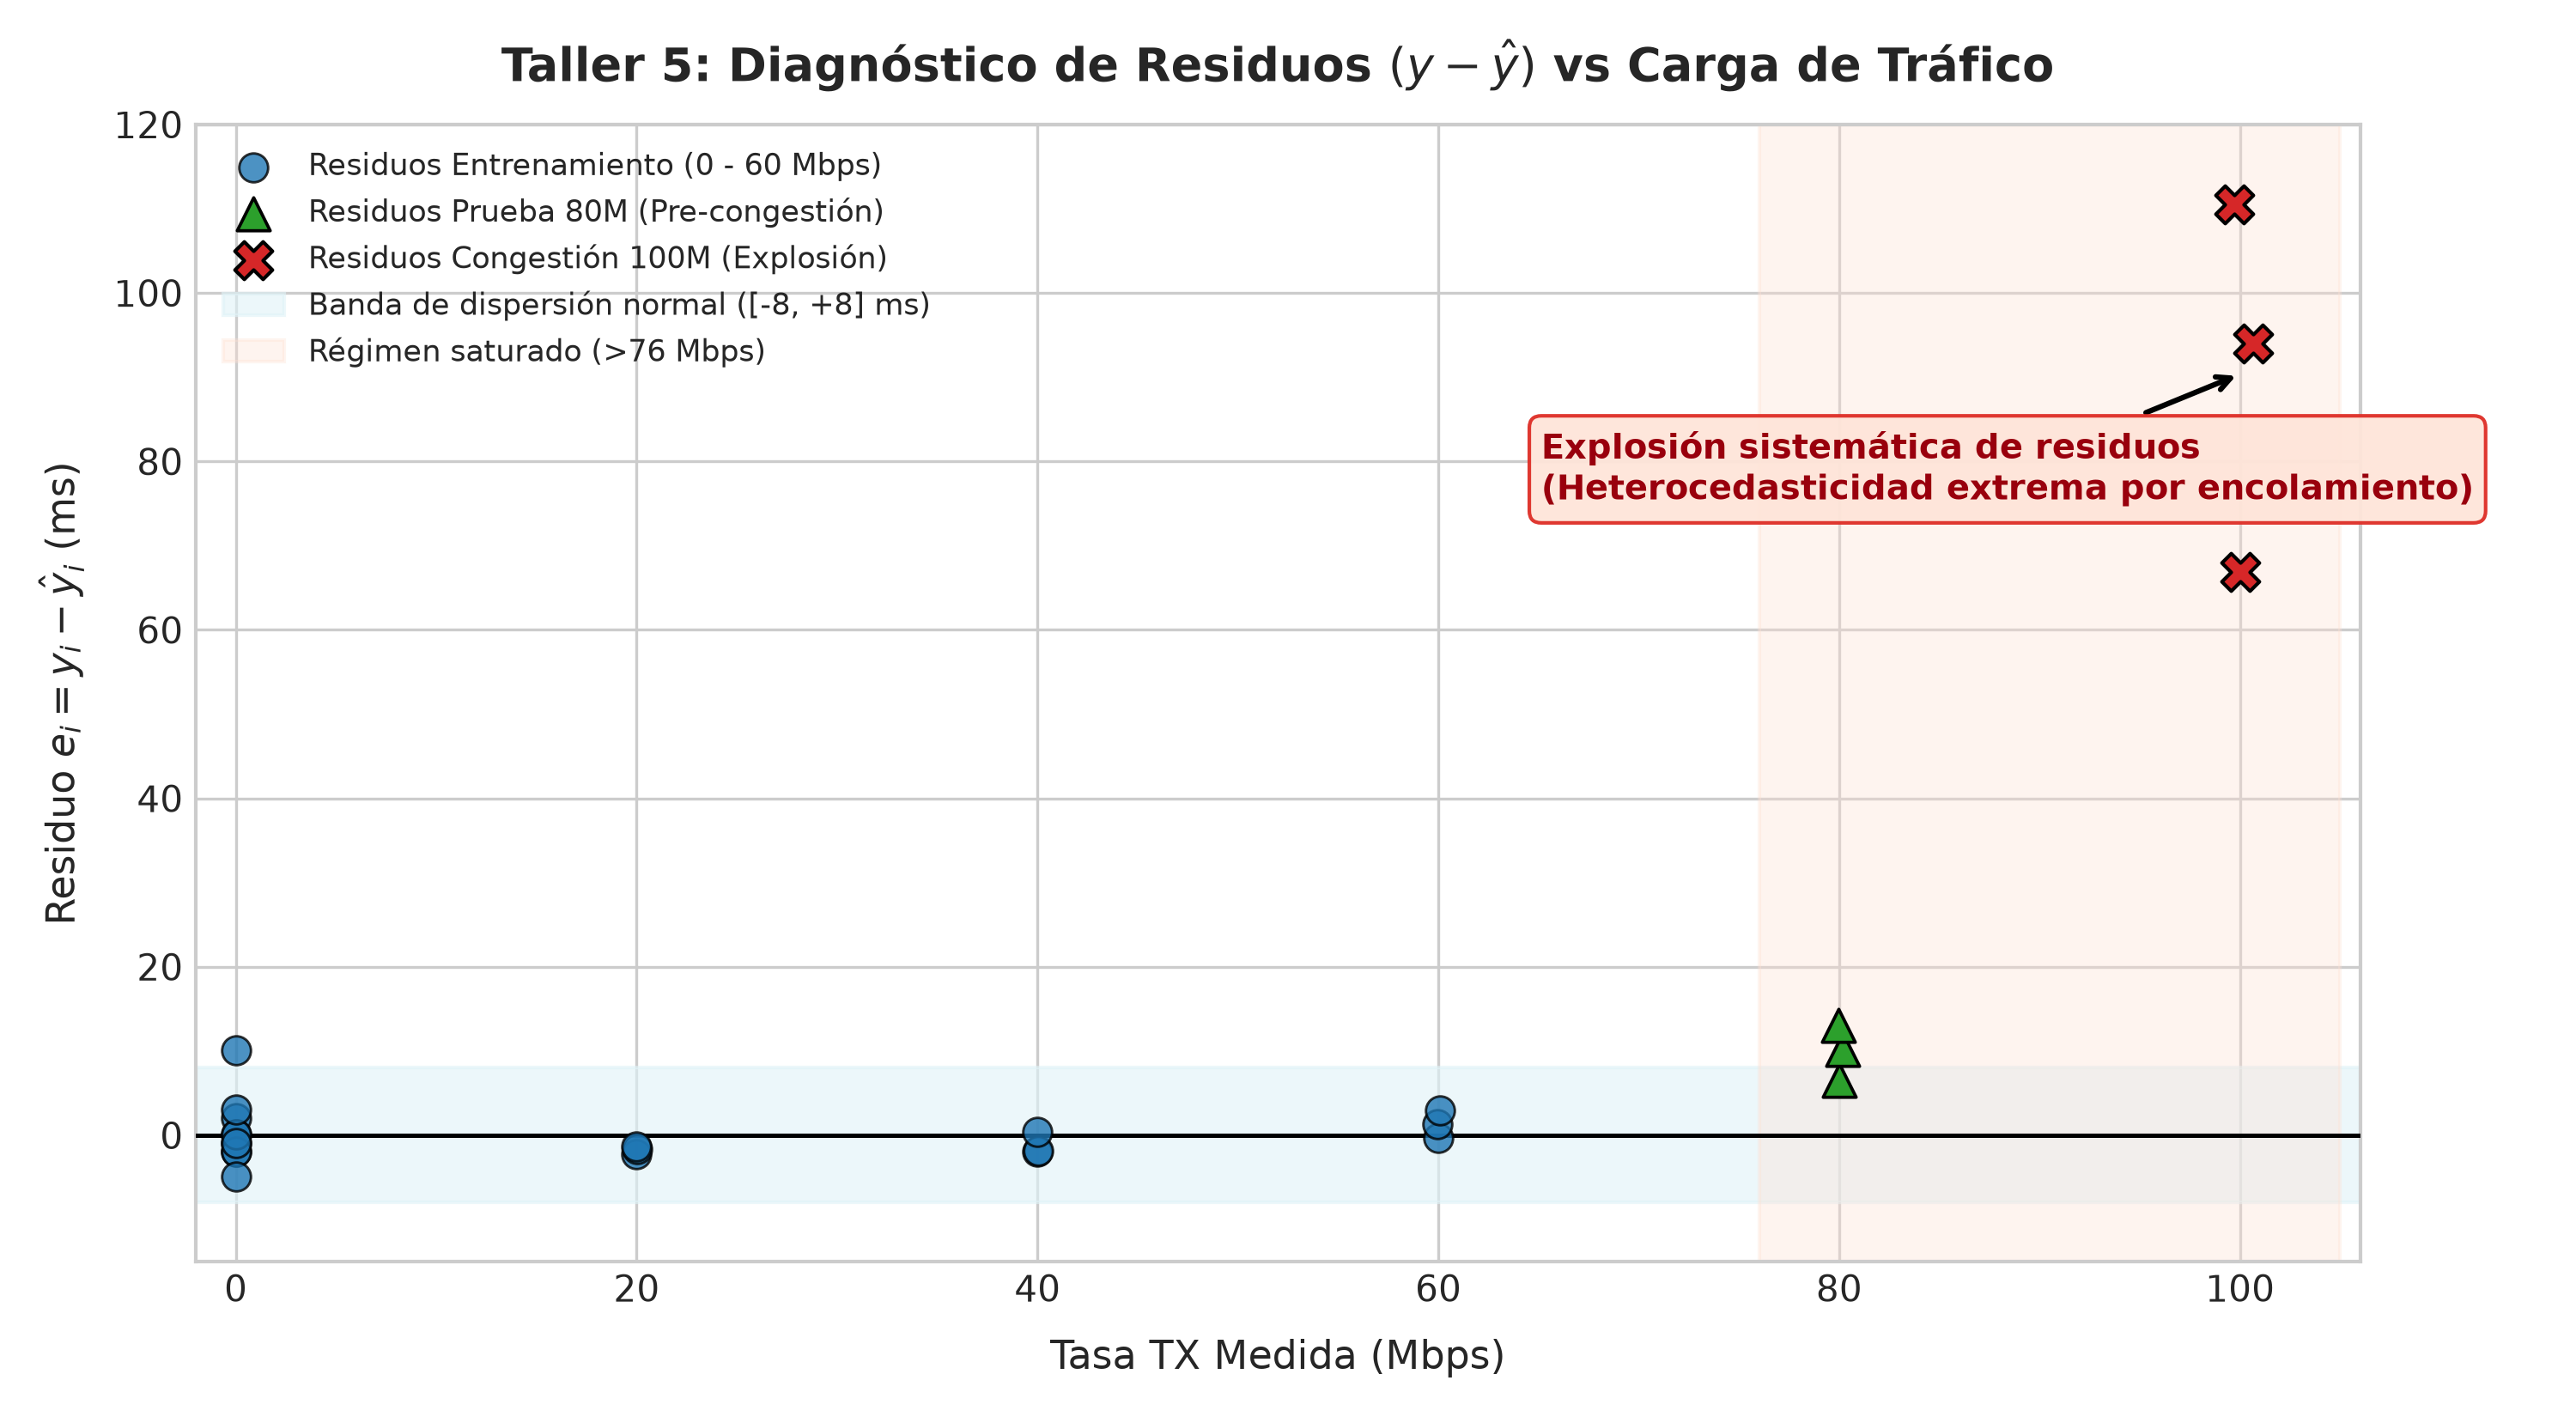
\includegraphics[width=\linewidth]{graficos/grafico6_analisis_residuos.png}
    \caption{Diagnóstico de residuos $(y - \hat{y})$ vs tasa TX.}
    \label{fig:residuos}
\end{figure}

\section{Predicción Bajo Congestión Severa y Límites (Evidencia 5)}

\subsection{Registro a Priori del Pronóstico en 100 Mbps}
Antes de contrastar con los datos empíricos de congestión, el modelo lineal entrenado en $[0, 60.07]\text{ Mbps}$ proyectó para una tasa $x \approx 100.13\text{ Mbps}$:
\begin{equation}
    \hat{y}_{100} = 13.9377 + 0.1755 \times (100.13) \approx \mathbf{31.51\text{ ms}}
\end{equation}
Dicha proyección constituyó una \textbf{extrapolación estricta} fuera del dominio de entrenamiento.

\subsection{Contraste Empírico y Diagnóstico de Ruptura}
Al confrontar el pronóstico con las 3 réplicas del escenario \texttt{05\_congestion\_100M} (Figuras \ref{fig:regresion} y \ref{fig:residuos}), se observó un desfase catastrófico:
\begin{itemize}
    \item \textbf{RTT Medido Real:} Mediana de $\mathbf{125.60\text{ ms}}$ (rango entre $98.40$ y $142.00\text{ ms}$).
    \item \textbf{Error Absoluto Medio (MAE):} $\mathbf{90.49\text{ ms}}$ (subestimación del $287.2\%$).
    \item \textbf{Residuo Sistemático:} $y - \hat{y} = [+66.92, +94.00, +110.56]\text{ ms}$.
\end{itemize}

\subsection{Respaldo Físico: El Fenómeno de Bufferbloat}
Las métricas telemétricas concurrentes confirman que la red ingresó en colapso por congestión:
\begin{enumerate}
    \item \textbf{Estancamiento del Caudal (\textit{Goodput}):} Mientras la tasa TX demandada fue de $100.13\text{ Mbps}$, el caudal efectivo recibido se estancó en $76.31\text{ Mbps}$, revelando la capacidad de cuello de botella del enlace.
    \item \textbf{Pérdida Crítica y Descartes:} Se registró un $22.23\%$ de pérdida de sondas y un total acumulado de $113{,}577$ paquetes descartados en las colas de conmutación.
\end{enumerate}

\subsection{Fundamento en Teoría de Colas y Modelo Segmentado}
La incapacidad del modelo lineal se explica por la teoría de colas $M/M/1$ de Kleinrock \cite{kurose2021computer}. En un encolador con tasa de servicio $\mu$ y tasa de llegada $\lambda$, el tiempo medio en el sistema es:
\begin{equation}
    W = \frac{1}{\mu - \lambda} = \frac{1/\mu}{1 - \rho}
\end{equation}
donde $\rho = \lambda / \mu$ es la utilización. Cuando $\lambda \to \mu$ ($\rho \to 1$), la latencia no crece de forma proporcional ($O(x)$), sino de forma hiperbólica hacia el infinito, acotada únicamente por el tamaño finito del búfer (\textit{Bufferbloat}). Una vez el búfer se llena, se produce descarte masivo (\textit{tail-drop}).

\textbf{Propuesta de Modelo Alternativo:} Se plantea restringir la regresión lineal únicamente a su rango de validez operacional ($x \le 75\text{ Mbps}$) y adoptar una \textit{Regresión Segmentada} (\textit{Piecewise Linear}):
\begin{equation}
    \hat{y}(x) = \begin{cases}
        \beta_0 + \beta_1 x, & \text{si } x \le x_{\text{codo}} \\
        (\beta_0 + \beta_1 x_{\text{codo}}) + \beta_2 (x - x_{\text{codo}})^2, & \text{si } x > x_{\text{codo}}
    \end{cases}
\end{equation}
donde $x_{\text{codo}} \approx 76\text{ Mbps}$ define el umbral de saturación.

\section{Respuestas a las Preguntas de Reflexión}

\subsection{Pregunta 1: ¿Por qué observar más bytes en A no necesariamente permite conocer la utilización total del switch?}
\noindent \textbf{Nota metodológica del laboratorio real:} En el banco de pruebas de este taller se utilizaron tres computadores personales (dos clientes A1 y A2, y un servidor receptor B) directamente interconectados en el mismo segmento LAN sin switch intermedio; por lo tanto, la saturación física residió en la interfaz de red (NIC) y búferes del servidor B.

\noindent No obstante, respondiendo al interrogante teórico sobre switches: Observar los contadores en la interfaz del equipo A mide únicamente el tráfico que atraviesa ese puerto de acceso específico. Un switch es una matriz de conmutación multipuerto (\textit{switching fabric}); si otros equipos (e.g. equipos C y D en otros puertos) transmiten tráfico simultáneo que satura la placa posterior (\textit{backplane}) o compite por el mismo búfer de salida compartida hacia el servidor B, el switch puede estar operando al 100\% de su capacidad de procesamiento global sin que el puerto A registre un volumen elevado de bytes. Además, contar bytes en A ignora tramas de broadcast, multicast de control o tráfico inter-VLAN ajeno al flujo observado.

\subsection{Pregunta 2: ¿Qué diferencia hay entre RTT medido con ping, latencia unidireccional y tiempo de respuesta de una aplicación?}
\begin{itemize}
    \item \textbf{RTT con \texttt{ping} (Capa 3 - ICMP):} Mide el tiempo total de ida y vuelta que le toma a un paquete IP viajar al destino y retornar. Está sujeto a priorización baja en el plano de control del kernel y no evalúa transporte ni puertos de aplicación.
    \item \textbf{Latencia Unidireccional (\textit{One-Way Delay} - OWD):} El tiempo que toma un paquete en viajar en un solo sentido ($A \to B$). Es asimétrica por naturaleza debido a diferencias de enrutamiento y requiere sincronización estricta de relojes (e.g. PTP o GPS).
    \item \textbf{Tiempo de Respuesta de Aplicación (Capa 7):} Incluye el RTT de red más el triple saludo TCP (3-way handshake), la negociación TLS/SSL, el tiempo de encolamiento en el servidor web y el tiempo de procesamiento de CPU y base de datos. Es significativamente mayor que el RTT de red puro.
\end{itemize}

\subsection{Pregunta 3: ¿Por qué un MAE pequeño bajo carga normal no garantiza acierto durante congestión?}
Un modelo ajustado en régimen no congestionado optimiza el error sobre una región donde la física del sistema es aproximadamente lineal y dominada por retardos fijos (propagación y transmisión). Un $MAE$ bajo en ese subespacio demuestra ajuste local, pero no garantiza capacidad de generalización fuera del dominio de soporte (\textit{out-of-distribution}). Cuando la red se satura, el régimen físico muta abruptamente hacia la teoría de colas no lineal. Como la derivada del retardo respecto a la carga se vuelve asintótica, el sesgo inductivo lineal genera un error de extrapolación inaceptable.

\subsection{Pregunta 4: ¿Cómo cambiaría el protocolo si los dispositivos se conectaran por Wi-Fi?}
Bajo Wi-Fi (IEEE 802.11):
\begin{enumerate}
    \item \textbf{Medio Compartido Semidúplex:} No es posible transmitir y recibir simultáneamente en el mismo canal.
    \item \textbf{Protocolo CSMA/CA y Contención:} En lugar de la conmutación dedicada de Ethernet, los nodos compiten mediante ventanas de contención y algoritmos de \textit{backoff} exponencial.
    \item \textbf{Sensibilidad a Ruido y Adaptación de Tasa (MCS):} La velocidad nominal fluctúa dinámicamente según la relación señal a ruido (SNR).
    \item \textbf{Impacto Metodológico:} La latencia basal $\beta_0$ sería sustancialmente más variable y con colas pesadas aún sin carga. El protocolo exigiría registrar métricas de retransmisiones a nivel de trama MAC, nivel de RSSI y canalización.
\end{enumerate}

\section{Conclusiones}
El Taller 5 demostró con éxito que los modelos lineales de Machine Learning son herramientas útiles y computacionalmente económicas para predecir la degradación de latencia en redes LAN bajo régimen operacional normal ($MAE \le 9.9\text{ ms}$). Sin embargo, se evidenció empírica y conceptualmente que la extrapolación lineal hacia regímenes de congestión severa carece de validez técnica ($MAE = 90.49\text{ ms}$), debido al fenómeno físico de \textit{Bufferbloat} y al comportamiento hiperbólico de las colas de conmutación.

\begin{thebibliography}{9}
\bibitem{hurbans2020grokking}
R. Hurbans, \textit{Grokking Artificial Intelligence Algorithms}, Manning Publications, 2020, Cap. 8: ``Machine Learning'', pp. 227--278.

\bibitem{kurose2021computer}
J. F. Kurose y K. W. Ross, \textit{Computer Networking: A Top-Down Approach}, 8th ed., Pearson, 2021.

\bibitem{kleinrock1975queueing}
L. Kleinrock, \textit{Queueing Systems, Volume 1: Theory}, Wiley-Interscience, 1975.
\end{thebibliography}

\end{document}
